%%========================================================================
%% LaTeX sjabloon voor stage/projectrapport of bachelorproef
%%  HoGent Bedrijf en Organisatie
%%========================================================================

%%========================================================================
%% Preamble
%%========================================================================

\documentclass[pdftex,a4paper,12pt,twoside]{report}

% XXX: Let op: dit sjabloon is gemaakt om dubbelzijdig af te drukken
% Voor enkelzijdig, verwijder ``twoside'' hierboven.

%%---------- Extra functionaliteit ---------------------------------------

\usepackage[utf8]{inputenc}  % Accenten gebruiken in tekst (vb. é ipv \'e)
\usepackage{amsfonts}        % AMS math packages: extra wiskundige
\usepackage{amsmath}         %   symbolen (o.a. getallen-
\usepackage{amssymb}         %   verzamelingen N, R, Z, Q, etc.)
%\usepackage[dutch]{babel}   % Taalinstellingen: woordsplitsingen,
                             %  commando's voor speciale karakters
                             %  ("dutch" voor NL)
\usepackage{eurosym}         % Euro-symbool €
\usepackage{geometry}
\usepackage{graphicx}        % Invoegen van tekeningen
\usepackage[pdftex,bookmarks=true]{hyperref}
                             % PDF krijgt klikbare links & verwijzingen,
                             %  inhoudstafel
\usepackage{epigraph}
\usepackage{listings}        % Broncode mooi opmaken
\usepackage{multirow}        % Tekst over verschillende cellen in tabellen
\usepackage{rotating}        % Tabellen en figuren roteren
\usepackage{natbib}          % Betere bibliografiestijlen
\usepackage{fancyhdr}        % Pagina-opmaak met hoofd- en voettekst

\usepackage[T1]{fontenc}     % Ivm lettertypes
\usepackage{lmodern}
\usepackage{textcomp}

%%---------- Layout ------------------------------------------------------

% hoofdingen, enz.
\pagestyle{fancy}
% enkel hoofdstuktitel in hoofding, geen sectietitel (vermijd overlap)
\renewcommand{\sectionmark}[1]{}

% lijn, wordt gebruikt in titelpagina
\newcommand{\HRule}{\rule{\linewidth}{0.5mm}}

% Leeg blad
\newcommand{\emptypage}{
\newpage
\thispagestyle{empty}
\mbox{}
\newpage
}

% Gebruik een schreefloos lettertype ipv het "oubollig" uitziende
% Computer Modern
\renewcommand{\familydefault}{\sfdefault}

% Commando voor invoegen Java-broncodebestanden (dank aan Niels Corneille)
% Gebruik: \codefragment{source/MijnKlasse.java}{Uitleg bij de code}
\newcommand{\codefragment}[2]{ \lstset{%
  language=java,
  breaklines=true,
  float=th,
  caption={#2},
  basicstyle=\scriptsize,
  frame=single,
  extendedchars=\true
}
\lstinputlisting{#1}}

%%---------- Documenteigenschappen ---------------------------------------
%% Vul dit aan met je eigen info:

% Je eigen naam
\newcommand{\student}{Jan {Van Braeckel}}

% De naam van je lector, begeleider, promotor
\newcommand{\promotor}{Joeri {Van Herreweghe}}

% De naam van je co-promotor
\newcommand{\copromotor}{Peter Leemans}

% Indien je bachelorproef in opdracht van een bedrijf of organisatie
% geschreven is, geef je hier de naam.
\newcommand{\instelling}{AllThingsTalk}

% De titel van het rapport/bachelorproef
\newcommand{\titel}{Bluetooth Low Energy wearables in een Internet of Things cloud-infrastructuur met behulp van een smartphone als gateway}
\newcommand{\titleEN}{Bluetooth Low Energy wearables in an Internet of Things cloud infrastructure using a smartphone as gateway}

% Datum van indienen
\newcommand{\datum}{29 mei 2015}

% Faculteit
\newcommand{\faculteit}{Faculteit `Bedrijf en Organisatie'}
\newcommand{\faculty}{Faculty `Bedrijf en Organisatie'}

% Soort rapport
\newcommand{\rapporttype}{Scriptie voorgedragen tot het bekomen van de graad\\Bachelor in de toegepaste informatica}
\newcommand{\reporttype}{Thesis submitted in fulfillment of the requirements for the degree of\\Bachelor in applied computer sciences}

% Academiejaar
\newcommand{\academiejaar}{2015-2016}

% Examenperiode
%  - 1e semester = 1e examenperiode
%  - 2e semester = 2e examenperiode
%  - tweede zit = 3e examenperiode
\newcommand{\examenperiode}{Tweede examenperiode}
\newcommand{\examperiod}{Second exam period}

%%========================================================================
%% Inhoud document
%%========================================================================

\begin{document}

%%---------- Front matter ------------------------------------------------
%% Het voorblad - Hier moet je in principe niets wijzigen.

\begin{titlepage}
  \newgeometry{top=2cm,bottom=1.5cm,left=1.5cm,right=1.5cm}
  \begin{center}

    \begingroup
    \rmfamily
    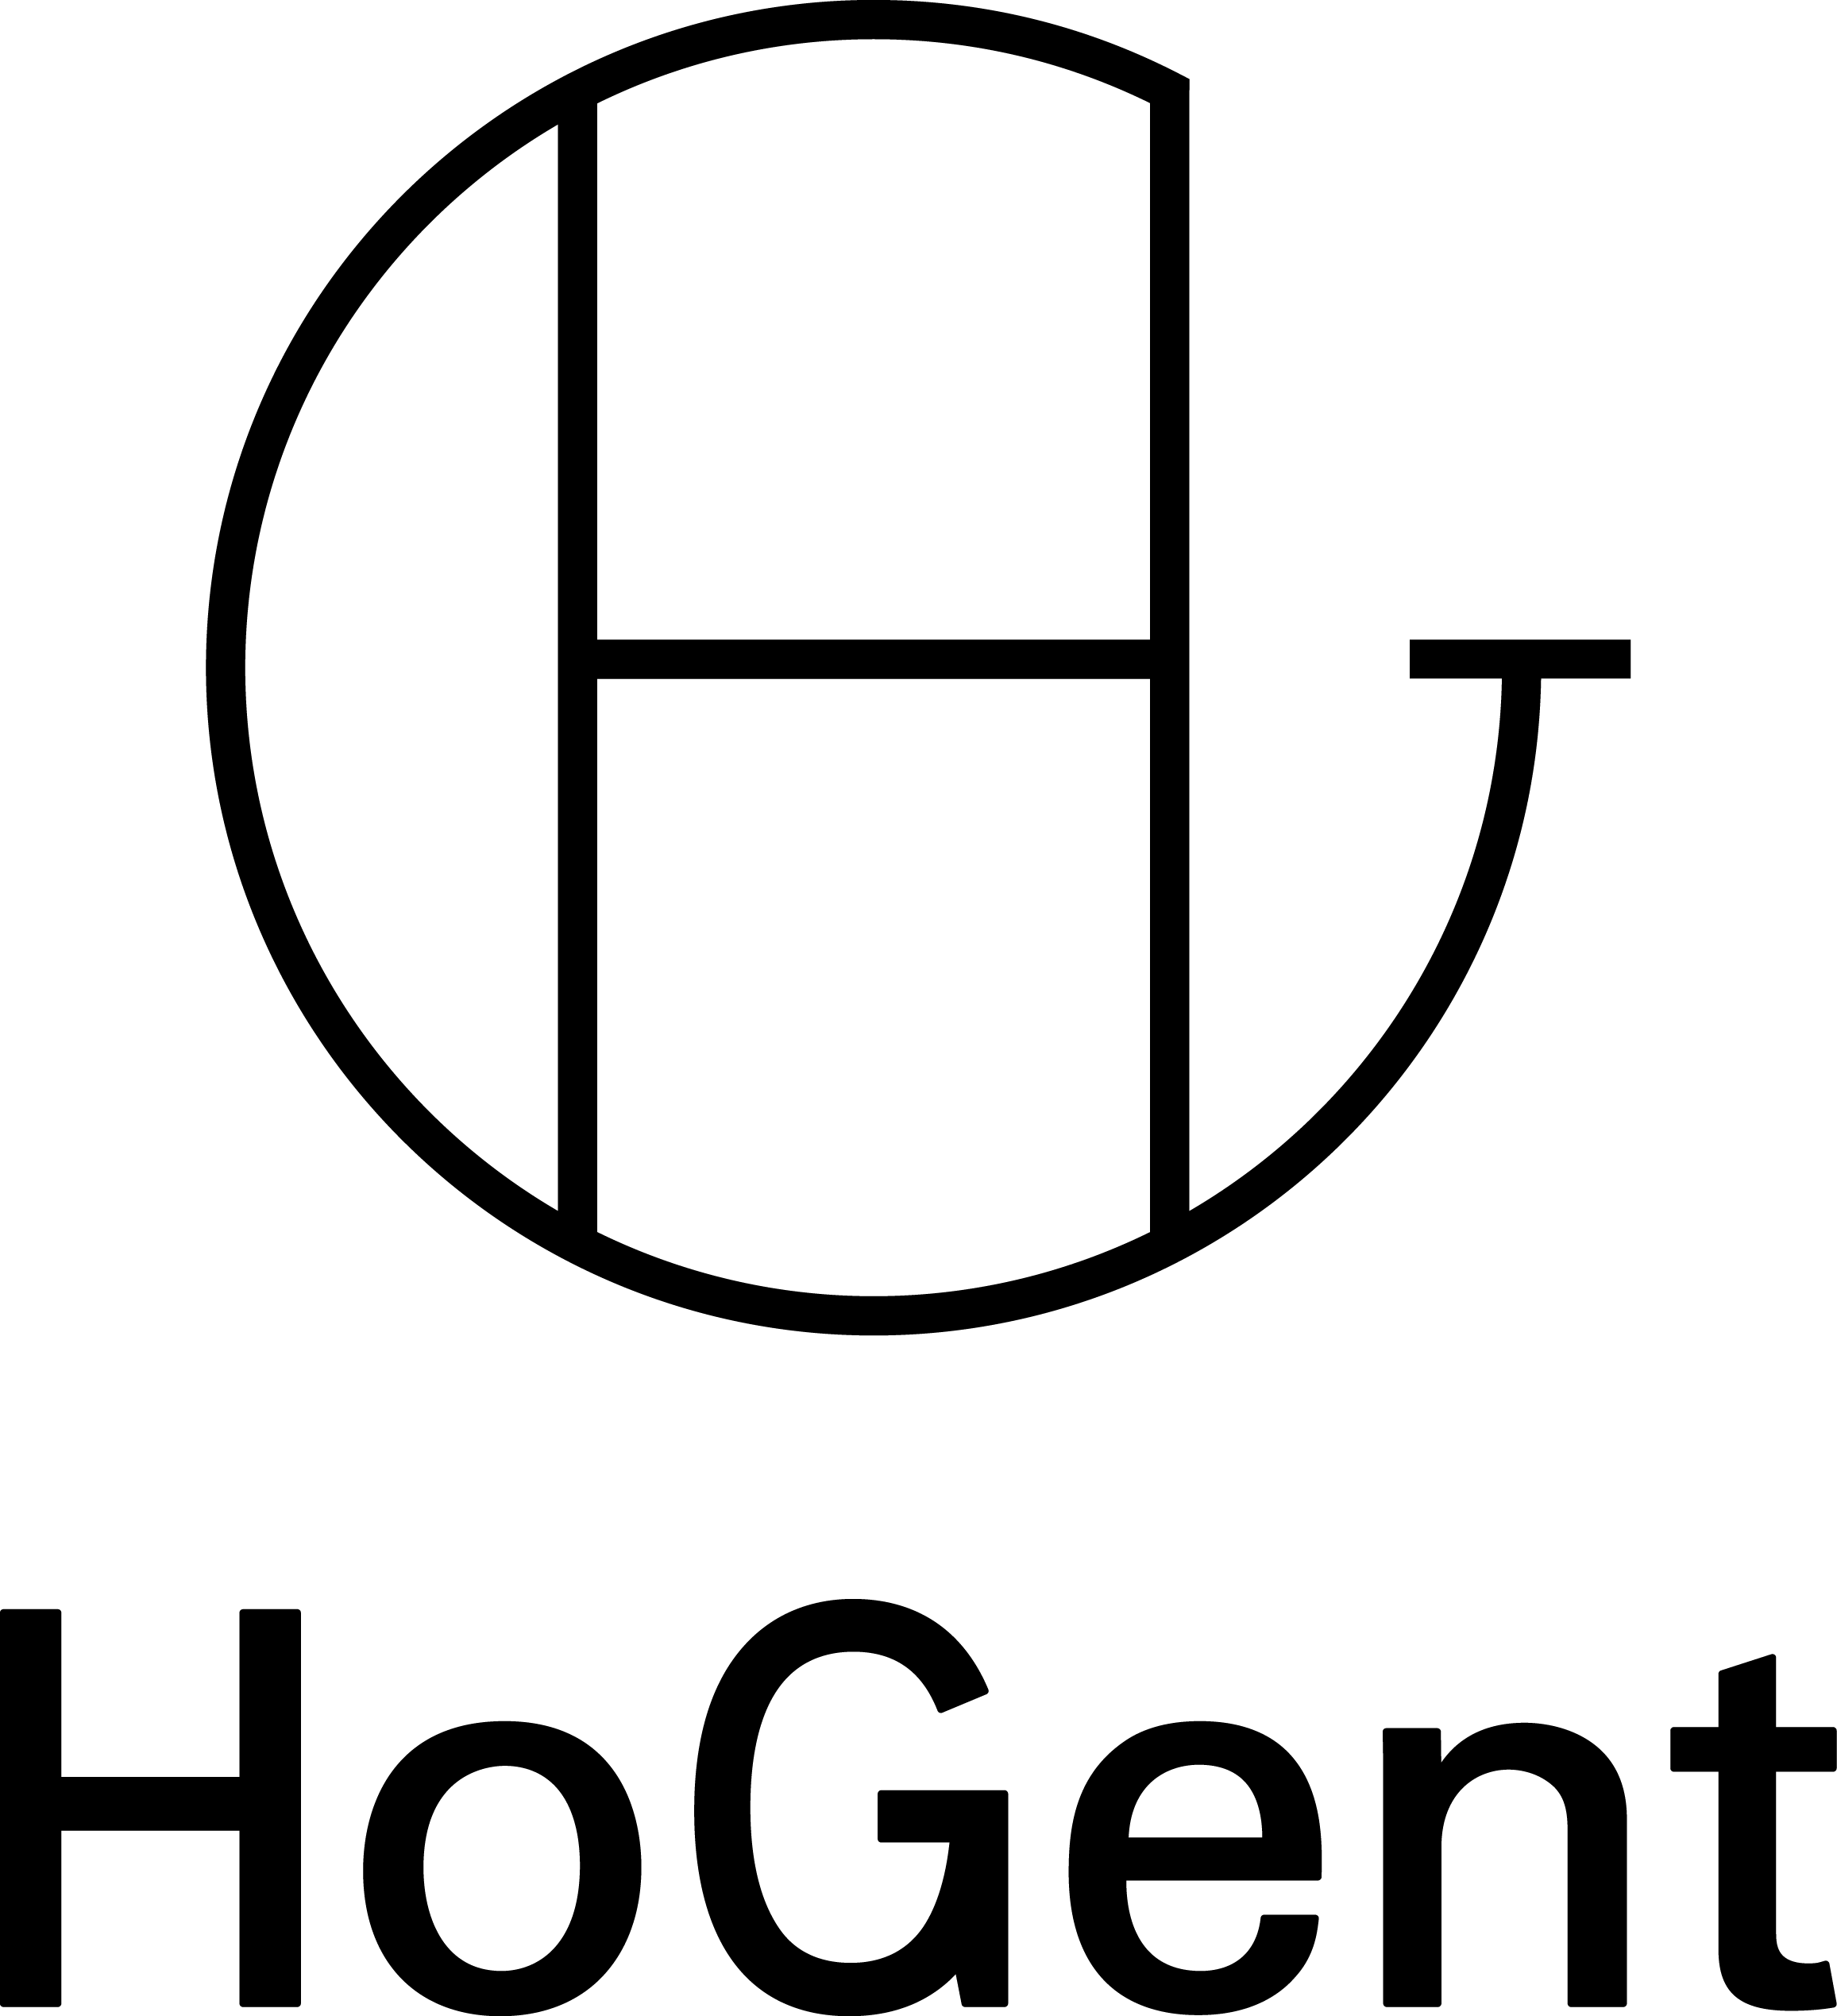
\includegraphics[width=2.5cm]{img/HG-beeldmerk-woordmerk}\\[.5cm]
    \faculteit\\[3cm]
    \titel
    \vfill
    \student\\[3.5cm]
    \rapporttype\\[2cm]
    Promotor:\\
    \promotor\\
    Co-promotor:\\
    \copromotor\\[2.5cm]
    Instelling: \instelling\\[.5cm]
    Academiejaar: \academiejaar\\[.5cm]
    \examenperiode
    \endgroup

  \end{center}
  \restoregeometry
\end{titlepage}

% Schutblad

\emptypage


\begin{titlepage}
  \newgeometry{top=5.35cm,bottom=1.5cm,left=1.5cm,right=1.5cm}
  \begin{center}

    \begingroup
    \rmfamily
    \faculty\\[3cm]
    \titleEN
    \vfill
    \student\\[3.5cm]
    \reporttype\\[2cm]
    Promoter:\\
    \promotor\\
    Co-promoter:\\
    \copromotor\\[2.5cm]
    Affiliation: \instelling\\[.5cm]
    Academic year: \academiejaar\\[.5cm]
    \examperiod
    \endgroup

  \end{center}
  \restoregeometry
\end{titlepage}


\begin{abstract}
% TODO: De "abstract" of samenvatting is een kernachtige (max 1 blz. voor een
% thesis) synthese van het document. In ons geval beschrijf je kort de
% probleemstelling en de context, de onderzoeksvragen, de aanpak en de
% resultaten.
\end{abstract}

\chapter*{Preface}
\label{ch:preface}

% TODO: Vergeet ook niet te bedanken wie je geholpen/gesteund/... heeft

\tableofcontents

% Als je een lijst van afkortingen of termen wil toevoegen, dan hoort die
% hier thuis. Gebruik bijvoorbeeld de ``glossaries'' package.

%%---------- Kern --------------------------------------------------------

\chapter{Introduction}
\label{ch:introduction}
\epigraph{If you think that the internet has changed your life, think again. The IoT is about to change it all over again!}{Brendan O'Brien}
The Internet of Things hasn't been around for a very long time, yet it's quickly becoming very popular and almost every tech company wants to be a part of it. It gained a lot of popularity around 2011 when IPV6 was released and it was around this time Gartner also took note of this technology and put it on their annual Hype Cycle for the first time. Around the same time of the growing popularity of the Internet of Things, the Bluetooth Special Interest Group also released a new Bluetooth specification that was built for the Internet of Things. Gartner suggests that by 2020, around 20 billion `things' will be connected to the Internet of Things, a market that Bluetooth Low Energy aims to play a big role in. This thesis aims to provide an introduction to Bluetooth Low Energy and how one would go about implementing Bluetooth Low Energy in the Internet of Things. In this chapter, the problem that the thesis is trying to find an answer for is elaborated, as well as the actual questions that need answering. An introduction about `AllThingsTalk' can also be found, a company that is trying to figure out how to include Bluetooth Low Energy wearables into their Internet of Things infrastructure.

% De inleiding moet de lezer alle nodige informatie verschaffen om het onderwerp te begrijpen zonder nog externe werken te moeten raadplegen \citep{Pollefliet2011}. Dit is een doorlopende tekst die gebaseerd is op al wat je over het onderwerp gelezen hebt (literatuuronderzoek).

% Je verwijst bij elke bewering die je doet, vakterm die je introduceert, enz. naar je bronnen. In \LaTeX{} kan dat met het commando \texttt{$\backslash${cite\{\}}} of \texttt{$\backslash${citep\{\}}}. Als argument van het commando geef je de ``sleutel'' van een ``record'' in een bibliografische databank in het Bib\TeX{}-formaat (een tekstbestand). Als je expliciet naar de auteur verwijst in de zin, gebruik je \texttt{$\backslash${}cite\{\}}.
% Soms wil je de auteur niet expliciet vernoemen, dan gebruik je \texttt{$\backslash${}citep\{\}}. Hieronder een voorbeeld van elk.

% \cite{Knuth1998} schreef een van de standaardwerken over sorteer- en zoekalgoritmen. Experten zijn het erover eens dat cloud computing een interessante opportuniteit vormen, zowel voor gebruikers als voor dienstverleners op vlak van informatietechnologie~\citep{Creeger2009}.
\newpage{}
\section{Problem statement and research questions}
\label{sec:problemdefinition}
In this section, the goal is to quickly familiarize you, the reader, with the subject this thesis is dealing about and which problems need to be solved in order to form a proper conclusion. First of all, the problem statement will be discussed where a quick sketch will be made as to why this thesis came to be. It will handle the problem AllThingsTalk is currently facing in the development of their company and why combining Bluetooth Low Energy with their Internet of Things infrastructure is the next logical step for their business. Next, we'll look at the main question AllThingsTalk wants an answer for together with some smaller questions that logically follow it.

\subsection{Problem statement}
\label{subsec:problemstatement}
At the time of writing, there are already a lot of Bluetooth enabled products on the technology market. With the new Bluetooth Low Energy specification, Bluetooth is reaching out even further to products like socks\footnote{http://www.sensoriafitness.com/}, shoes\footnote{https://secure-nikeplus.nike.com/plus/products/basketball}, fitness bands\footnote{https://www.fitbit.com/} and more are being added to the list every day. The problem with these products is that in a lot of cases, the products only synchronize with a smartphone. Some manufacturers extend this connectivity by occasionally synchronizing the data the smartphone captures to their own proprietary cloud, where the data can be analyzed by both the company and the consumer. Most of the time, this is where the data cycle stops and it can't be further accessed by other parties, this is known as a closed loop system. In some cases, developers can still access the data with an API that communicates with the cloud service of the manufacturer, but this doesn't give any access to the raw sensor values and doesn't allow real-time data transfer.

On top of this, a lot of the devices being manufactured don't use standard SIG adopted BLE services, which makes interoperability with existing applications hard, if not impossible if authentication and encryption are added into the mix.

\subsection{Research questions}
\label{subsec:researchquestions}
There are a couple of questions that can be asked when combining Bluetooth Low Energy and the Internet of Things, and some of those questions alone could have multiple papers dedicated. For example, the matter of security will be a never ending debate, and even more concerns arise when talking about security in the Internet of Things. These security concerns will be addressed further in section \ref{sec:concerns}. Another concern is privacy, but since this is very much a gray area, it's hard to formulate a one-sided conclusion on this matter.

The main goals this thesis tries to fulfill are in essence very simple, but of course there are always some other questions that arise when looking at the big picture. These questions can be categorized as following, the questions in bold being the main research questions and the ones in plain text being auxiliary questions:
\begin{itemize}
	\item{\textbf{Can Bluetooth Low Energy wearables be used in an Internet of Things cloud infrastructure?}}
	\item{\textbf{Is is possible to use a smartphone as gateway to communicate with the AllThingsTalk cloud in real-time?}}
	\item{What is Bluetooth Low Energy?}
	\item{What is the difference between Bluetooth Low Energy and Bluetooth Classic?}
	\item{What are the pros and cons of this technology?}
	\item{What types of devices exist in Bluetooth Low Energy and how do they expose their data?}
\end{itemize}

\section{AllThingsTalk}
\label{sec:allthingstalk}

% TODO: Wees zo concreet mogelijk bij het formuleren van je
% onderzoeksvra(a)g(en). Een onderzoeksvraag is trouwens iets waar nog
% niemand op dit moment een antwoord heeft (voor zover je kan nagaan).

\chapter{Methodology}
\label{ch:methodology}

% TODO: Hoe ben je te werk gegaan? Verdeel je onderzoek in grote fasen, en
% licht in elke fase toe welke stappen je gevolgd hebt. Verantwoord waarom je
% op deze manier te werk gegaan bent. Je moet kunnen aantonen dat je de best
% mogelijke manier toegepast hebt om een antwoord te vinden op de
% onderzoeksvraag.


%% TODO: de structuur en titel van deze hoofdstukken hangen af van je
% eigen onderzoek. Elke fase in je onderzoek kan een eigen hoofdstuk krijgen. Kies telkens een gepaste titel. ``Corpus'' is *GEEN* gepaste titel
\chapter{Bluetooth Low Energy}
\label{ch:ble}

\section{What is Bluetooth Low Energy}
\label{sec:whatis}

\section{Key differences between classic Bluetooth}
\label{sec:differencesclassic}

\subsection{A new technology emerges}
\label{subsec:newtechnology}

\subsection{Limitations of Bluetooth Low Energy}
\label{subsec:limitations}

\section{Bluetooth configurations}
\label{sec:bleconfigurations}

\section{How low energy is achieved}
\label{sec:lowenergy}

\chapter{The Bluetooth Low Energy protocol stack}
\label{sec:protocolstack}

\section{Controller}
\label{sec:stackController}

\subsection{Physical Layer}
\label{subsec:controllerPHY}

\subsection{Link Layer}
\label{subsec:controllerLL}

\subsection{Host Controller Interface}
\label{subsec:controllerHCI}

\section{Host}
\label{sec:stackHost}

\subsection{Host Controller Interface}
\label{subsec:hostHCI}

\subsection{Logical Link Control and Adaption Protocol}
\label{subsec:hostATTL2CAP}

\subsection{Attribute Protocol}
\label{subsec:hostATT}

\subsection{Security Manager Protocol}
\label{subsec:hostSMP}

\subsection{Generic Access Profile}
\label{subsec:hostGAP}

\subsection{Generic Attribute Profile}
\label{subsec:hostGATT}

\section{Application}
\label{sec:stackApplication}

\subsection{Application}
\label{subsec:applicationApp}

\chapter{Generic Access Profile}
\label{ch:gap}

\chapter{Generic Attribute Profile}
\label{ch:gatt}

\section{Profiles}
\label{sec:profiles}

\section{Services}
\label{sec:services}

\section{Characteristics}
\label{sec:characteristics}

\section{Descriptors}
\label{sec:descriptors}

\chapter{Why Bluetooth Low Energy and Internet of Things}
\label{ch:BLEIOT}

\chapter{Android programming}
\label{ch:android}

\chapter{Discussion}
\label{ch:discussion}

\section{Conclusion}
\label{sec:conclusion}

\section{Concerns}
\label{sec:concerns}

\section{Further research}
\label{sec:furtherresearch}

% TODO: Trek een duidelijke conclusie, in de vorm van een antwoord op de
% onderzoeksvra(a)g(en). Reflecteer kritisch over het resultaat. Zijn er
% zaken die nog niet duidelijk zijn? Heeft het ondezoek geleid tot nieuwe
% vragen die uitnodigen tot verder onderzoek?



\bibliographystyle{apa}
\bibliography{tin-bachproef}

%%---------- Back matter -------------------------------------------------

\listoffigures
\listoftables

\end{document}
